\documentclass[aps,twocolumn,showpacs]{revtex4-1}


\usepackage{epsfig}
\usepackage{amsfonts}
\usepackage{amssymb}
\usepackage{mathrsfs}
\usepackage{theorem}
\usepackage{amsmath}
\usepackage{times}
\usepackage{color}
\usepackage[french]{babel}
\usepackage[T1]{fontenc}
\usepackage{ifpdf}
\ifpdf
\usepackage{epstopdf}   
\usepackage{url}
\fi


\begin{document}
\title{Novel detection of spin interactions in diamond}

\author{Clément Pellet-Mary$^1$, Maxime Perdriat$^1$, Paul Huillery$^1$, and Gabriel Hétet$^{1}$}
\email{gabriel.hetet@phys.ens.fr}
\affiliation{$^1$Laboratoire de physique de l'ENS, ENS Paris, France\\
}

\begin{abstract}
\normalsize
NV$^-$ centers in diamond are a widely used quantum system, both for applications and fundamental research, thanks to their good coherence properties, long lifetimes and most importantly their ability to be optically polarized.
We have recently found new ways to use these properties of NV centers in order to study the dipolar interactions between ensemble of spins in diamond, including NV centers as well as other spin defects. 

On one part, we have observed cross-relaxations (CR) between NV centers and other defects (see Fig. 1), namely VH- \cite{VH}, War1 (first defect found by EPR at the university of Warwick, still chemically unknown) and $^{13}$C First-shell modified NV. None of these defects had been observed through CR before. This is a first step toward hyper-polarization of new spin defects in diamond.

On another part, we have used the mechanical detection of a levitating diamond to measure the torque applied by the NV centers on the diamond when two classes of NV with different orientation are put to resonance(see Fig. 2). We have linked this effect to the dipolar-mediated modification of the T$_1$ of NV centers happening with dense ensembles.\cite{Lukin}. This paves the way toward the mechanical detection of other spin impurities in diamond, as well as the observation of the Einstein-de Haas effect with paramagnetic systems. \cite{Meriles}

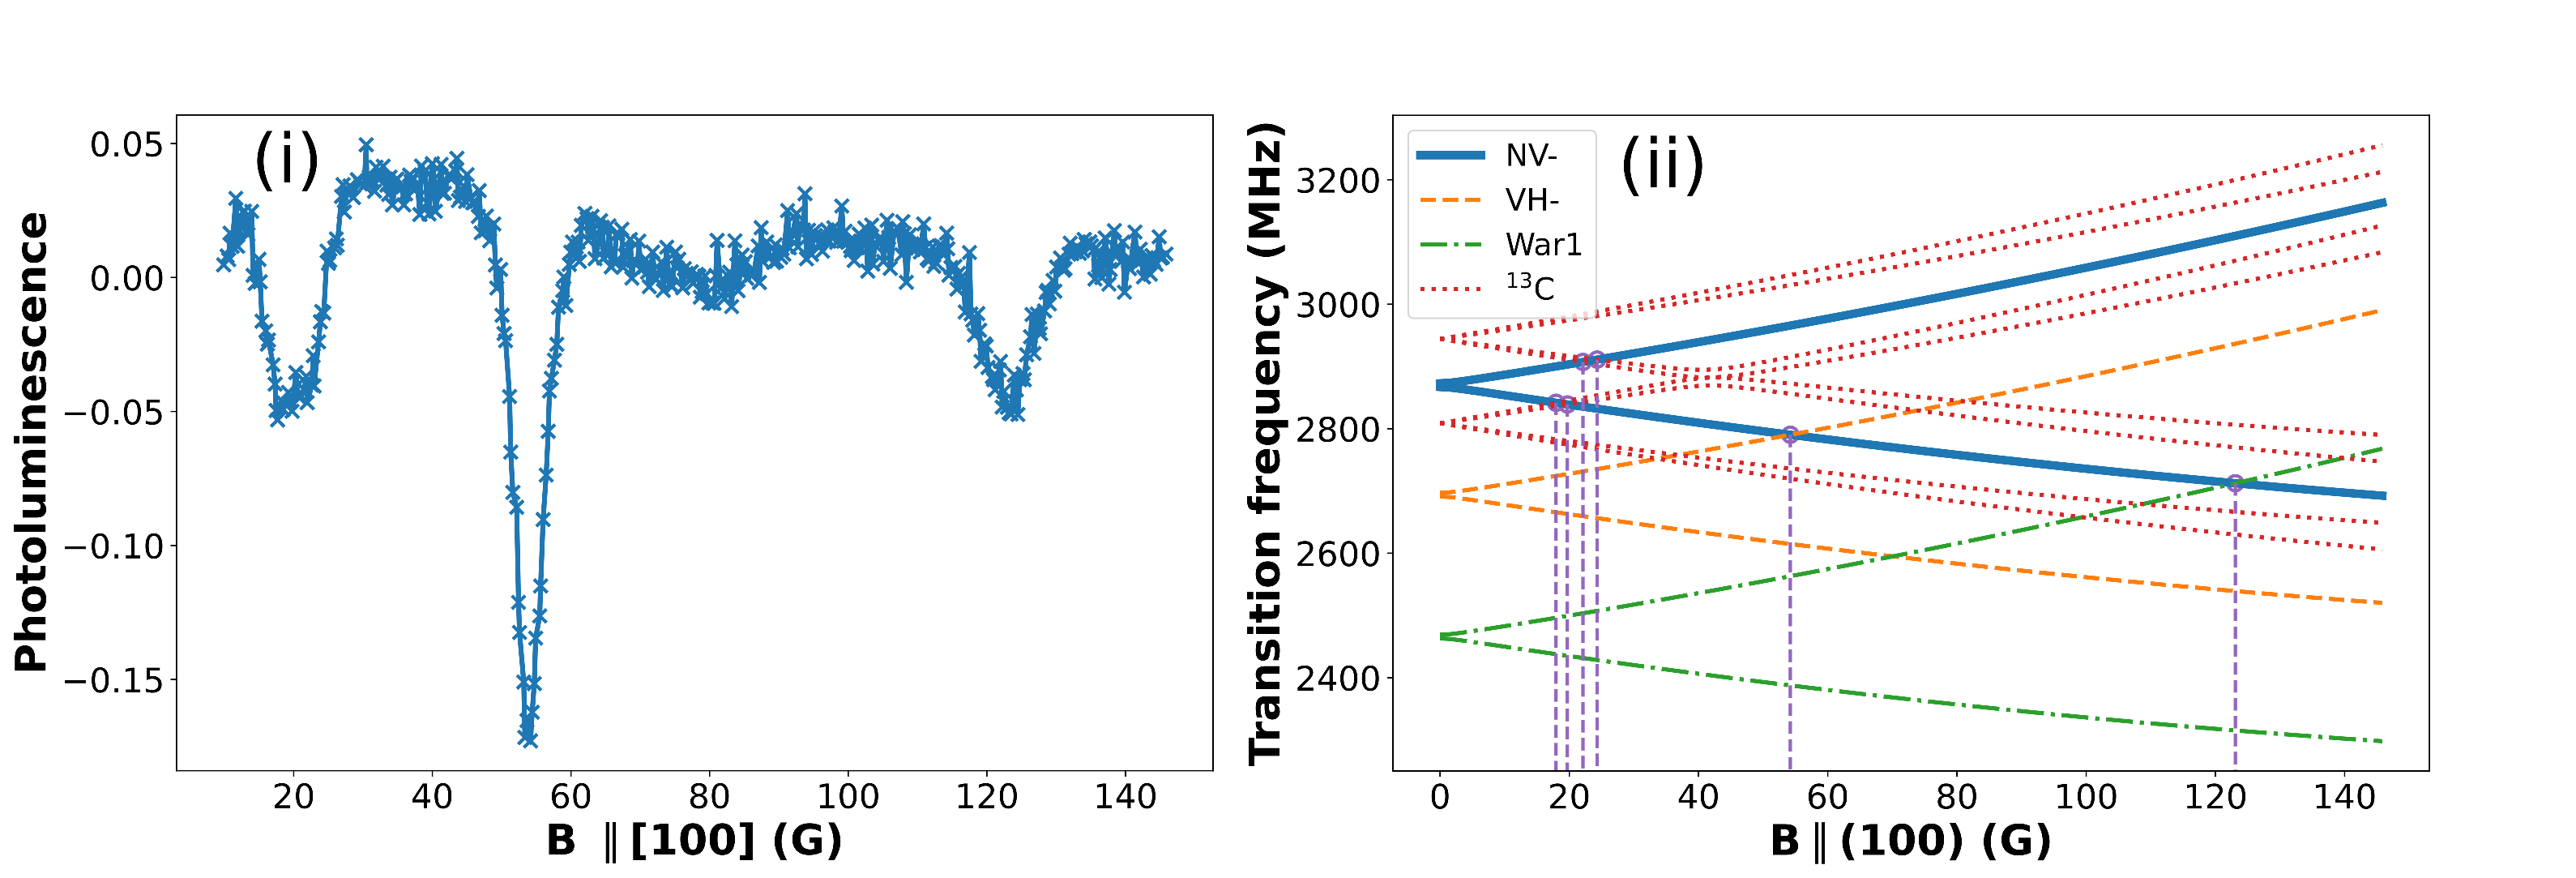
\includegraphics[scale=.25]{CR_total}
Figure 1 : i) Photoluminescence change while scanning the magnetic field along the crystalline [100] direction. ii) Energy levels for various species : Plain : NV centers, dotted : NV centers with hyper-fine coupling of a first-shell $^{13}$C, dashed : VH$^-$, dash-dotted : War1. The predicted cross relaxation with NV centers are at 18-24 G for first-shell $^{13}$C, 54 G for VH$^-$ and 123 G for War1

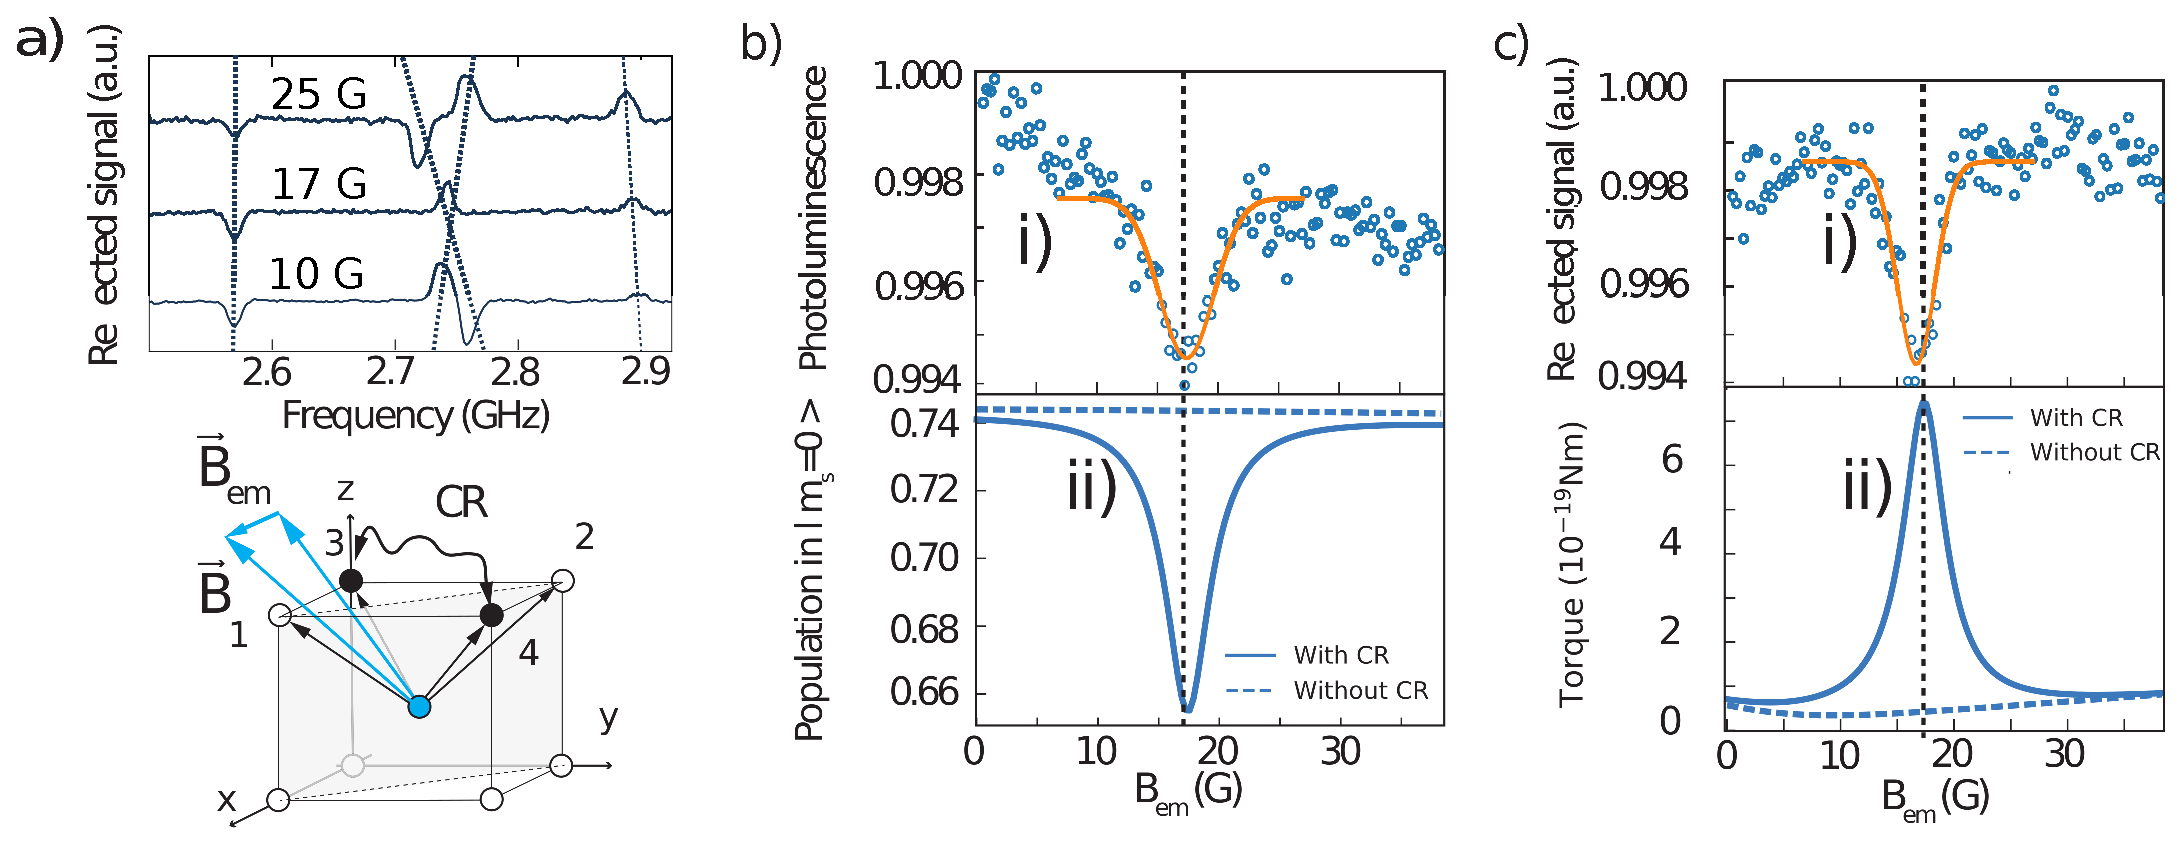
\includegraphics[scale=.5]{CRmeca}
Figure 2 : i) ESR spectra while scanning B$_{em}$ with some bias field applied. ii)Angular position of the diamond while scanning B$_{em}$ without a microwave. The rotation of the diamond at 17 G corresponds to the resonance between two classes of NV
\end{abstract}

\maketitle

\begin{thebibliography}{}

\bibitem{VH} Glover, Claire, et al. "Hydrogen incorporation in diamond: The nitrogen-vacancy-hydrogen complex." Physical review letters 90.18 (2003): 185507.

\bibitem{Lukin} Choi, Joonhee, et al. "Depolarization dynamics in a strongly interacting solid-state spin ensemble." Physical review letters 118.9 (2017): 093601.

\bibitem{Meriles} Zangara, Pablo R., et al. "Mechanical rotation via optical pumping of paramagnetic impurities." Physical Review B 100.23 (2019): 235410.

\end{thebibliography}
\end{document}
